% options:
% thesis=B bachelor's thesis
% thesis=M master's thesis
% czech thesis in Czech language
% english thesis in English language
% hidelinks remove colour boxes around hyperlinks

\documentclass[thesis=B,english]{FITthesis}[2012/10/20]

% \usepackage[utf8]{inputenc} % LaTeX source encoded as UTF-8
% \usepackage[latin2]{inputenc} % LaTeX source encoded as ISO-8859-2
% \usepackage[cp1250]{inputenc} % LaTeX source encoded as Windows-1250

\usepackage{graphicx} %graphics files inclusion
% \usepackage{subfig} %subfigures
% \usepackage{amsmath} %advanced maths
% \usepackage{amssymb} %additional math symbols

\usepackage{dirtree} %directory tree visualisation
\usepackage{listings}
\usepackage{verbatim}

% % list of acronyms
% \usepackage[acronym,nonumberlist,toc,numberedsection=autolabel]{glossaries}
% \iflanguage{czech}{\renewcommand*{\acronymname}{Seznam pou{\v z}it{\' y}ch zkratek}}{}
% \makeglossaries

% % % % % % % % % % % % % % % % % % % % % % % % % % % % % % 
% EDIT THIS
% % % % % % % % % % % % % % % % % % % % % % % % % % % % % % 
\setcounter{tocdepth}{2}
\department{Department of Software Engineering}
\title{Adobe Premiere Pro Plugin for NARRA}
\authorGN{Dmitry} %author's given name/names
\authorFN{Vanyagin} %author's surname
\author{Dmitry Vanyagin} %author's name without academic degrees
\authorWithDegrees{Dmitry Vanyagin} %author's name with academic degrees
\supervisor{Ing. Petr Pulc}
\acknowledgements{I would like to thank my supervisor Ing. Petr Pulc for his help, support and guidance and Michal Moc{\v n}{\' a}k for providing of a working instance of NARRA.}
\abstractEN{This bachelor thesis describes a process of development of a plug-in for Adobe Premiere Pro CC. Main goal is to allow user to communicate with NARRA web API directly from Adobe Premiere Pro interface. User will be able to browse lists of accessible footage, import it and synchronize metadata. Result of this work is an application that fulfills the requirements and can be used as a basis for future development, that provides intuitive and responsive user interface.}
\abstractCS{V n{\v e}kolika v{\v e}t{\' a}ch shr{\v n}te obsah a p{\v r}{\' i}nos t{\' e}to pr{\' a}ce v {\v c}esk{\' e}m jazyce.}
\placeForDeclarationOfAuthenticity{Prague}
\keywordsCS{Replace with comma-separated list of keywords in Czech.}
\keywordsEN{NARRA, Adobe Premiere Pro CC, RESTful API, Panel SDK, ExtendScript, Plug-in}
\declarationOfAuthenticityOption{1} %select as appropriate, according to the desired license

\graphicspath{ {./IMAGES/} }
\lstdefinelanguage{JavaScript}{
  	keywords={typeof, new, true, false, catch, function, return, null, catch, switch, var, if, in, while, do, else, case, break},
  	keywordstyle=\bfseries,
 	ndkeywords={class, export, boolean, throw, implements, import, this},
 	ndkeywordstyle=\bfseries,
 	sensitive=false,
 	comment=[l]{//},
 	morecomment=[s]{/*}{*/},
 	commentstyle=\ttfamily,
  	stringstyle=\ttfamily,
 	morestring=[b]',
	morestring=[b]"
}

\lstset{
   	language=JavaScript,
   	extendedchars=true,
   	basicstyle=\footnotesize\ttfamily,
   	showstringspaces=false,
   	showspaces=false,
   	numbers=left,
   	numberstyle=\footnotesize,
  	numbersep=9pt,
   	tabsize=2,
   	breaklines=true,
   	showtabs=false,
   	captionpos=b
}

\begin{document}

% \newacronym{CVUT}{{\v C}VUT}{{\v C}esk{\' e} vysok{\' e} u{\v c}en{\' i} technick{\' e} v Praze}
% \newacronym{FIT}{FIT}{Fakulta informa{\v c}n{\' i}ch technologi{\' i}}

\setsecnumdepth{part}
\chapter{Introduction}
The possibility to visualize and annotate data is always been appreciated in circles of people, who works with a huge amounts of information every day. NARRA is a software that provides this functionality for those using large amounts of video in their practice – artists collaborating on open narratives, video editors, social scientists using video as a research tool, documentary filmmakers with expanded projects. 

Artists can tell stories together using video. Instead of a linear narrative, media works can have multiple paths, multiple versions. The software can be used to create, visualize and navigate a tree of linked stories.

Video editors faced with hundreds of hours of material can annotate their media objects and then organize it based on complex search categories. The software itself will use existing software libraries to add functionality and perform automated annotations. For example the software can extract spoken words and make them into attached text; list shot size, geographic location, etc.

The main purpose of this thesis is to create a tool to use all this functionality and communicate with NARRA directly from your computer. I chose to implement it as a plug-in for Adobe Premiere Pro video editing software application. This application is widely used by different broadcasters such as the BBC\cite{bbc} and CNN\cite{cnn}, also many people chose it as a part or their workflow. Using this plug-in user will be able to directly communicate with NARRA API, i.e., to import and export sequences of clips with all attached metadata. 

To develop this tool I will use mainly Adobe Premiere Pro SDK and Third-party libraries for solving arising problems or for extending functionality provided by SDK.
\setsecnumdepth{all}
\chapter{Analysis}
\section{Requirements specification}
\subsection{Functional requirements}
Final product have to fulfill basic requirements:
	\begin{description}
		\item [Authorization in NARRA] 
User should be able to authorize in NARRA, get a token that will be used for all transactions between plug-in and NARRA API. Since Google and Github identities are used inside NARRA, plug-in should communicate with those authorization services.
		\item [Displaying a list of projects]
User should be able to browse a list of his projects inside NARRA.
		\item [Displaying a list of libraries]
User should be able to browse a list of his libraries inside NARRA.
		\item [Displaying a list of items]
User should be able to browse a list of his items inside NARRA.
		\item [Searching an item]
Plug-in should provide convenient search input field for a user to search an item in a list.
		\item [Importing items from NARRA to Adobe Premiere Pro]
User should be able to choose an item from his project list and import it in the Adobe Premiere Pro.
		\item [Pushing changes of metadata of an item to NARRA]
User should be able to synchronize all metadata changes made in item with NARRA.
		\item [Synchronization of item metadata between NARRA and local machine]
Plug-in should support synchronization of item metadata between NARRA and Adobe Premiere Pro project.
		\item [Plug-in appearance should mimic design of Adobe Premiere Pro itself]
Plug-in's appearence should look like it is a part of user interface and it should change color scheme accordingly to color scheme of Adobe Premiere Pro.
	\end{description}
\subsection{Non-Functional requirements}
	\begin{itemize}
		\item User interface should be clear and understandable for a user.
		\item Plug-in should work in Adobe Premiere Pro CS5.5 and newer versions.
		\item Internet connection is required to use all functionality.
	\end{itemize}
\section{Use cases}
In this section I will try to describe the basic use cases for this application. In order to communicate with NARRA, user has to complete authorization process, that's why almost every use case require user to be logged in. You can see use case diagram on figure \ref{fig:usecase}.
	\begin{description}
		\item[Authorization in NARRA] 
User wants to authorize himself in order to use plug-in. After plug-in launch, user has to choose an authorization method (choose entity provider). There is two possibilities:
	\begin{itemize}
		\item Authorization using Google account.
		\item Authorization using Github account.
	\end{itemize}
After user clicks on one of these buttons, system default web browser will be launched and user will be redirected to a login page of chosen entity provider. On this page user enters his/her credentials and submits the form. After successful authorization, user's access token will be displayed. This token has to be copied by user to an input field in the plug-in and submitted. 
		\item[Browsing project list] 
User can see a list of his/her projects in NARRA. Requirements: User has to be logged in. There are several way how to access project list:
	\begin{itemize}
		\item After successful authorization, list of projects that given user contributes to will be displayed. 
		\item User can click "Projects" menu button to get to the list of projects from any part of the plug-in.
	\end{itemize}
		\item[Browsing library list] 
User can see a list of his/her libraries in NARRA. Requirements: User has to be logged in. There are several way how to access library list:
	\begin{itemize}
		\item After successful authorization, list of projects that given user contributes to will be displayed, user clicks on the desired project to see which libraries this project contain. List of libraries appears. 
		\item User can click "Libraries" menu button to get to the list of libraries from any part of the plug-in.
	\end{itemize}
		\item[Import new item from NARRA]
User wants to import an item from NARRA. Requirements: User has to be logged in. Basic scenario:
	\begin{enumerate}
		\item User selects item to download.
		\item User clicks on download option. Default browser launches and user sees all information about given item.
		\item User clicks download button. Downloading of .zip archive starts.
		\item User unzips archive and "drag and drops" contents of this archive into project bin inside Premiere Pro.
	\end{enumerate}
		\item[Editing of metadata]
User wants to edit project metadata and save changes back to NARRA. User can add metadata using Adobe Premiere Pro tools. Requirements: User has to be logged in. Basic scenario:
	\begin{enumerate}
		\item User edits metadata of an item inside project bin using Adobe Premiere Pro tools.
		\item User clicks "sync" button. Plugin synchronizes items with NARRA.
	\end{enumerate}
		\item[Searching for an item]
User wants to find a specific item in his item list. Requirements: User has to be logged in. Basic scenario: 
	\begin{enumerate}
		\item User enters the keyword in a search field.
		\item User clicks search button or presses "Enter" key. List of items will be refreshed displaying search results.
	\end{enumerate}
		\item [Changing colorscheme]
User wants to change color scheme of Adobe Premiere Pro interface. User does that via settings dialog provided by Premiere Pro. Plug-in changes it's color scheme accordingly.
		\item [User logout]
User wants to work from another account. Basic scenario:
	\begin{enumerate}
		\item User clicks on "Logout" button. User gets redirected to login screen, information about his token removed from plug-in.
		\item User chooses the method of authorization by clicking on a button. Default browser opens up and displays authorization from provided by chosen service.
		\item User provides his/her credentials and submits the form. Authorization token is displayed.
		\item User copies token to input field on plug-in login page and clicks "Login". Token is saved inside plug-in and user is redirected to project list. 
	\end{enumerate}
	\end{description}
	\begin{figure}
		\centering
		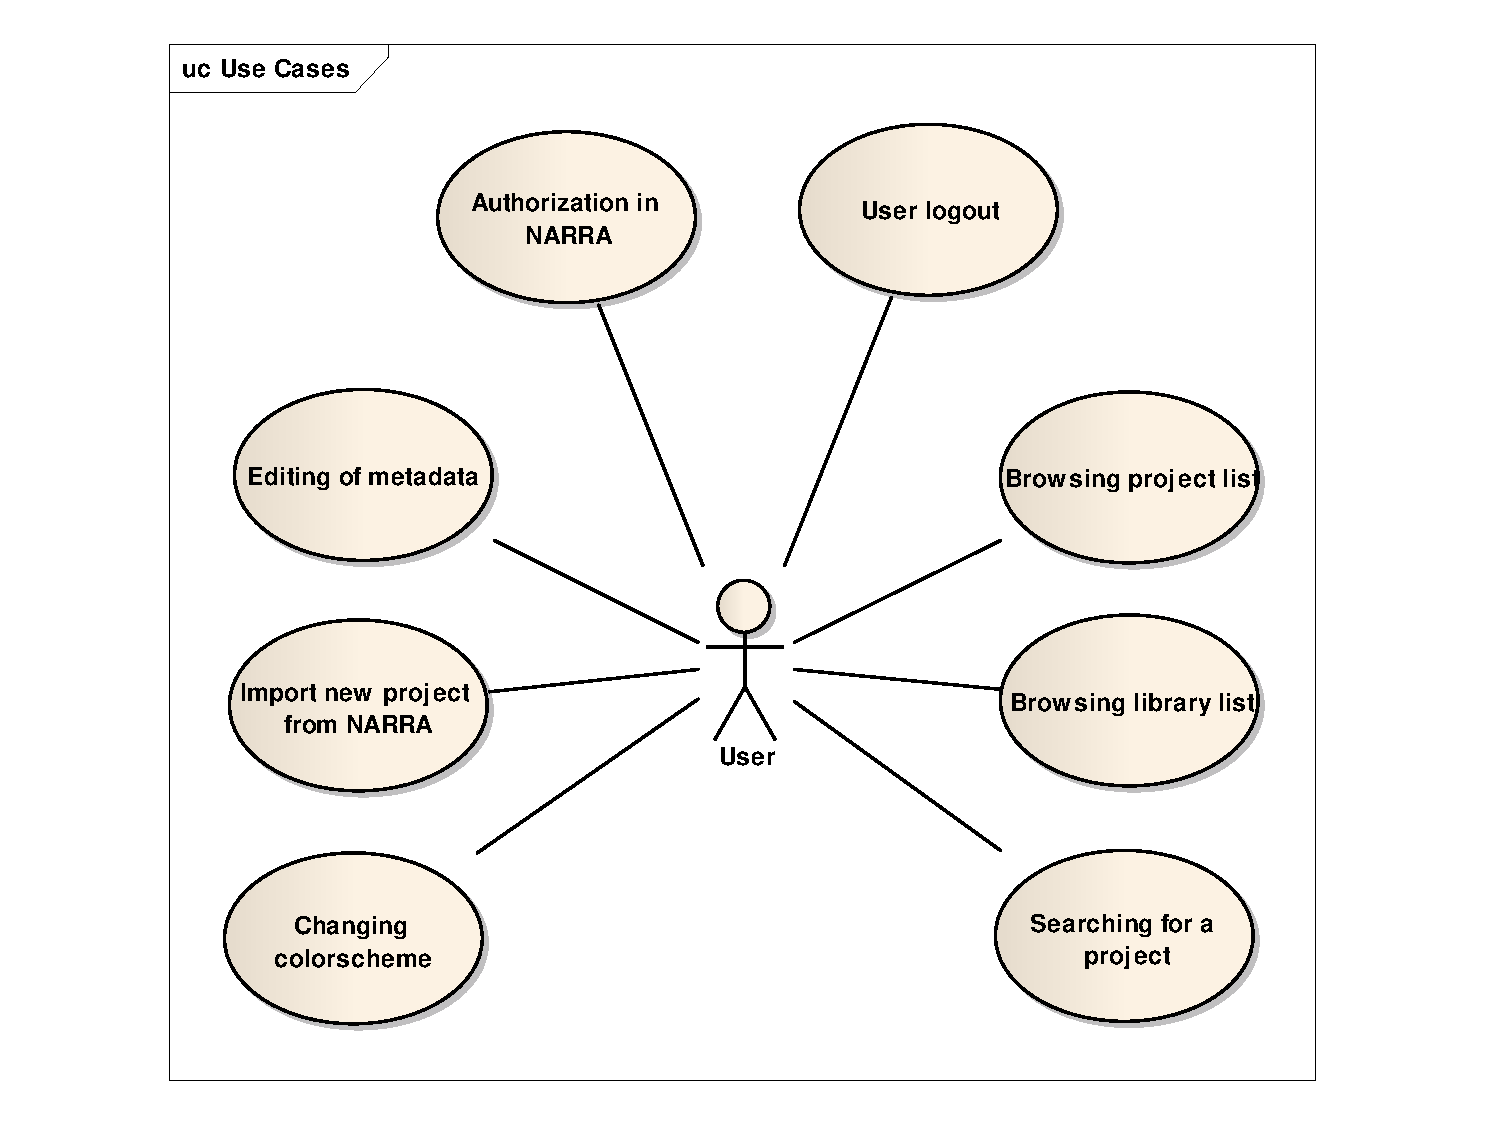
\includegraphics[width=1\textwidth]{UseCases.pdf}
		\caption{Use case diagram}\label{fig:usecase}
	\end{figure}
\section{Structure of application}
I decided to split this application into two plug-ins:
	\begin{itemize}
		\item Import plug-in (Importer).
		\item Export plug-in (Exporter).
	\end{itemize}
The reason why I chose this structure is because it is more logical to have two lightweight plug-ins that solve it's own task. If user wants to import a project into Adobe Premiere Pro, he/she can launch Importer, to export a project Exporter can be used. On figure \ref{fig:narrastruct} you can see a sketch of communication between application and NARRA, you can see that plug-in directly uses Adobe Premiere Pro SDK and communicates with NARRA using http protocol. All video files are stored in a cloud storage.
	\begin{figure}
		\centering
		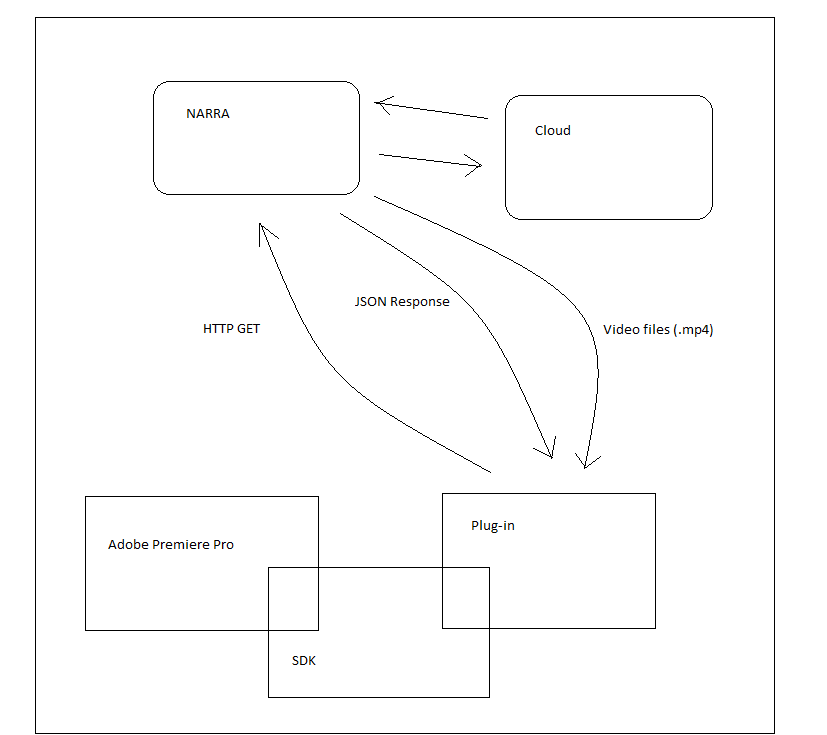
\includegraphics[width=1\textwidth]{StructureofNARRA.png}
		\caption{Sketch of communication with NARRA}\label{fig:narrastruct}
	\end{figure}

\section{Web API}
I this section I would like to describe a layer between our plug-in and NARRA. At first I will analyze different methods of building web API like SOAP and REST, compare them and then I will write about particular implementation of NARRA API.

\textbf{Application programming interface} (API) is a set of routines, protocols, and tools for building software applications. An API expresses a software component in terms of its operations, inputs, outputs, and underlying types. An API defines functionalities that are independent of their respective implementations, which allows definitions and implementations to vary without compromising each other.

\subsection{SOAP}
SOAP is an XML language defining a message architecture and message formats, hence providing a rudimentary processing protocol. The SOAP document defines a toplevel XML element called envelope, which contains a headerand a body. The SOAP header is an extensible container for message-layer infrastructure information that can be used for routing purposes (e.g., addressing) and Quality of Service (QoS) configuration (e.g., transactions, security, reliability). The body contains the payload of the message. XML Schema is used to describe the structure of the SOAP message, so that SOAP engines at the two endpoints can marshall and unmarshall the message content and route it to the appropriate implementation.

\textbf{Web Services Description Language} (WSDL) is an XML language for defining interfaces syntactically. A WSDL port type contains multiple abstract operations, which are associated with some incoming and outgoing messages. The WSDL binding links the set of abstract operations with concrete transport protocols and serialization formats. By default, there is no notion of state. The interaction with stateful Web services is covered by the WS-Resource Framework, which handles the management of stateful resources behind a Web service interface.

	\begin{description}
		\item[Strength of SOAP] 
SOAP message format and the WSDL interface definition language have gained popularity as the technologies capable of delivering interoperability between systems. One advantage is protocol transparency and independence.

Using SOAP, the same message in the same format can be transported across a variety of  systems, which may rely on HTTP, but also on many other transports. The transport protocol may change along the way.

Using WSDL to describe a service interface helps to abstract from the underlying communication protocol and serialization details as well as from the service implementation platform (operating system and programming language). WSDL contracts provide a machine-processable description of the syntax and structure of the corresponding request and response messages and define a flexible evolution path for the service. 

As business and technology requirements change, the same abstract service interface can be bound to different transport protocols and messaging endpoints. In particular, WSDL can model service interfaces for systems based on synchronous and asynchronous interaction patterns.\cite{soaprest}
		\item[Weaknesses of SOAP] 
Paradoxically, the power of SOAP can also be misused. Thus, it is important to avoid leakage across abstraction levels. Interoperability problems can occur when, for instance, native data types and language constructs of the service implementation are present in its interface.\cite{soaprest}

The translation between the XML and the corresponding memory data structures has been problematic and is the main source of performance inefficiencies. Furthermore, XML Schema is a very rich language, making it difficult to identify the right construct to express a data model in a way that is fully supported by all SOAP/WSDL implementations.\cite{soaprest}
	\end{description}
\subsection{REST}
REpresentational State Transfer (REST) was originally introduced as an architectural style for building large-scale distributed hypermedia systems.

The REST architectural style is based on four principles:
	\begin{description}
		\item[Resource identification through URI.] A RESTful Web service exposes a set of resources which identify the targets of the interaction with its clients. Resources are identified by URIs, which provide a global addressing space for resource and service discovery. 			
		\item[Uniform interface.] Resources are manipulated using a fixed set of four create, read, update, delete operations: PUT, GET, POST, and DELETE. PUT creates a new resource, which can be then deleted using DELETE. GET retrieves the current state of a resource in some representation. POST transfers a new state onto a resource.\cite{soaprest}
		\item[Self-descriptive messages.] Resources are decoupled from their representation so that their content can be accessed in a variety of formats (e.g., HTML, XML, plain text, PDF, JPEG, etc.). Metadata about the resource is available and used, for example, to control caching, detect transmission errors, negotiate the appropriate representation format, and perform authentication or access control. 
		\item[Stateful interactions through hyperlinks.] Every interaction with a resource is stateless, i.e., request messages are self-contained. Stateful interactions are based on the concept of explicit state transfer. Several techniques exist to exchange state, e.g., URI rewriting, cookies, and hidden form fields. State can be embedded in response messages to point to valid future states of the interaction.\cite{soaprest}
	\end{description}
Now I want to describe strengths and weaknesses of REST:
	\begin{description}
		\item[Strength of REST] 
RESTful Web services are designed to be simple. HTTP clients and servers are available for all major programming languages and operating system/hardware platforms, and the default HTTP port 80 is commonly left open by default in most firewall configurations. Such lightweight infrastructure, is inexpensive to acquire and thus has a very low barrier for adoption.

The effort required to build a client to a RESTful service is very small as developers can begin testing such services from an ordinary Web browser, without having to develop custom client-side software.\cite{soaprest} 

Deploying a RESTful Web service is very similar to building a dynamic Web site. Furthermore, thanks to URIs and hyperlinks, REST has shown that it is possible to discover Web resources without an approach based on compulsory registration to a (centralized) repository. On the operational side, it is known how to scale a stateless RESTful Web service to serve a very large number of clients, thanks to the support for caching, clustering and load balancing built into REST. Due to the possibility of choosing lightweight message formats, e.g., the JavaScript Object Notation (JSON) or, even plain text for very simple data types, REST also gives more possibilities to optimize the performance of a Web service.
		\item[Weaknesses of REST] 
There is some confusion regarding the commonly accepted best practices for building RESTful Web services. Recommendations have been established informally. 

Most of the REST services uses just GET and POST (first for idempotent requests, second for everything else) because some proxies and firewalls may not always allow connections that use other method.
These restrictions have led to a series of workarounds, where the "real" verb is sent using either a special HTTP header (X-HTTP-Method-Override). As with most non-standard workarounds, these may not be understood by all Web servers, and require additional development and testing effort. Another limitation makes it impossible to strictly follow the GET vs. POST rule. For idempotent requests having large amounts of input data (more than 4 KB in most current implementations) it is not possible to encode such data in the resource URI, as the server will reject such URI or in the worst case it will crash, exposing the service to buffer overflow attacks. The size of the request notwithstanding, it may also be challenging to encode complex data structures into a URI as there is no commonly accepted marshalling mechanism. Inherently, the POST method does not suffer from such limitations.\cite{soaprest}
	\end{description}
\subsection{NARRA API}
NARRA API is designed following RESTful approach, HTTP protocol is used to communicate with it. I would like to describe basic requests and responses that will be useful for our plug-in:
	\begin{itemize}
		\item \textbf{Authentication} \cite{api_auth}

In order to access resources of NARRA and use it's functionality, user has to be logged in and present with an access token. Authentication request can be  initialized by following URL: 

\texttt{GET auth/google}

User will be redirected to authentication page of Google. After successful submission of the form user will be present with an access token:
\begin{verbatim}
{"status":"OK","token":"MTRzNjc2MhAxNDYzORk0NTgwAjUv"}
\end{verbatim}
At least first request to NARRA API has to contain copy this token in data payload.

		\item \textbf{User profile} \cite{api_profile}

To get information about currently signed in user, this URL should be used:

\texttt{GET v1/users/me}

Response might look like following:

\begin{verbatim}
{"status":"OK","user":{
  "username":"bob",
  "name":"Bob Example",
  "email":"bob@example.org",
  "image":"https://lh3.googleusercontent.com/.../photo.jpg?sz=50",
  "roles":["author","admin"],
  "identities":["google"]}
}
\end{verbatim}

		\item \textbf{Items} \cite{api_items}

Item is the individual video clip, image, sound file or any piece of data supported by NARRA. To get information about items this URL should be used:

\texttt{GET v1/items}

Result might look like following:
\label{toc:api_items}
\begin{verbatim}
{"status":"OK","items":[
  {"id":"552a33df61633249940c0000",
   "name":"00129O-051",
   "url":"http://example.org/00129O-051.mov",
   "type":"video",
   "prepared":true,
   "thumbnails":[
    "http://narra-storage/.../thumbnail_00000.png"
   ],
   "video_proxy_hq":
    "http://narra-storage/.../video_proxy_hq.webm",
   "video_proxy_lq":
    "http://narra-storage/.../video_proxy_lq.webm",
   "audio_proxy":
    "http://narra-storage/.../audio_proxy.ogg"},
  {"id":"552a33df61633276b1090000",
   "name":"0013D2-013-2",
   "url":"http://example.org/0013D2-013-2.mov",
   "type":"video",
   "prepared":true,
   "thumbnails":[
    "http://narra-storage/.../thumbnail_00000.png",
    "http://narra-storage/.../thumbnail_00004.png"
   ],
   "video_proxy_hq":
    "http://narra-storage/.../video_proxy_hq.webm",
   "video_proxy_lq":
    "http://narra-storage/.../video_proxy_lq.webm",
   "audio_proxy":
    "http://narra-storage/.../audio_proxy.ogg"}
]}
\end{verbatim}

		\item \textbf{Specific item}

In order to get information about specific item this URL should be used:

\texttt{GET v1/items/552a33df61633249940c0000}

Result might look like following:
\begin{verbatim}
{"status":"OK","item":{
  "id":"552a33df61633249940c0000",
  "name":"00129O-051",
  "url":"http://example.org/00129O-051.mov",
  "type":"video",
  "prepared":true,
  "library":{"id":"552a328961633276b1000000","name":"Example Library"},
  "thumbnails":[
   "http://narra-storage/.../thumbnail_00000.png"
  ],
  "video_proxy_hq":
   "http://narra-storage/.../video_proxy_hq.webm",
  "video_proxy_lq":
   "http://narra-storage/.../video_proxy_lq.webm",
  "audio_proxy":
   "http://narra-storage/.../audio_proxy.ogg",
  "metadata":[]
}}
\end{verbatim}

		\item \textbf{Libraries}

Libraries are used to organize items into easily manageable units. In order to get information about libraries this URL should be used:

\texttt{GET v1/libraries}

Response might look like following:
\begin{verbatim}
{"status":"OK","libraries":[
  {"id":"5538da453533632e3c060000",
   "name":"Example Library",
   "description":"This is an example",
   "author":{"username":"alice","name":"Alice Example"},
   "thumbnails":[
    "http://narra-storage/.../thumbnail_00012.png",
    "http://narra-storage/.../thumbnail_00006.png",
    "http://narra-storage/.../thumbnail_00018.png",
    "http://narra-storage/.../thumbnail_00030.png",
    "http://narra-storage/.../thumbnail_00024.png"
   ],
   "contributors":[{"username":"bob","name":"Bob Example"}]},
  {"id":"5838da453533632e3c060000",
   "name":"My example",
   "description":"This is my example",
   "author":{"username":"bob","name":"Bob Example"},
   "thumbnails":[
    "http://narra-storage/.../thumbnail_00006.png",
    "http://narra-storage/.../thumbnail_00012.png",
   ],
   "contributors":[]}
]}
\end{verbatim}

		\item \textbf{Specific library}

To list information about specific library this URL should be used:

\texttt{GET v1/libraries/5538da453533632e3c060000}

Response might look like following:
\begin{verbatim}
{"status":"OK","library":{
  "id":"5538da453533632e3c060000",
  "name":"Example Library",
  "description":"This is an example",
  "generators":[
   {"identifier":"att_speech",
    "title":"AT&T Speech To Text",
    "description":"Speech To Text Generator"}
  ],
  "author":{"username":"alice","name":"Alice Example"},
  "thumbnails":[
   "http://narra-storage/.../thumbnail_00012.png",
   "http://narra-storage/.../thumbnail_00006.png",
   "http://narra-storage/.../thumbnail_00018.png",
   "http://narra-storage/.../thumbnail_00030.png",
   "http://narra-storage/.../thumbnail_00024.png"
  ],
  "contributors":[{"username":"bob","name":"Bob Example"}],
  "projects":[
   {"id":"552a31cd6163324994020000",
    "name":"my_project",
    "title":"Example Project",
    "author":{"username":"bob","name":"Bob Example"}}
   ],
  "metadata":[
   {"name":"Location","value":"FAMU"},
   {"name":"Source","value":"SD_0320"}
  ]
}}
\end{verbatim}

		\item \textbf{Projects}

Project is the highest level of item organization, it's role is to keep organized all data involved in single piece of audiovisual work. To list all accessible projects this URL should be used:

\texttt{GET v1/projects}

Response might look like following:
\begin{verbatim}
{"status":"OK","projects":[
  {"name":"my_project",
   "title":"Example Project",
   "description":"This is an example project.",
   "author":{"username":"bob","name":"Bob Example"},
   "public":"false",
   "thumbnails":[
    "http://narra-storage/.../thumbnail_00012.png",
    "http://narra-storage/.../thumbnail_00020.png",
    "http://narra-storage/.../thumbnail_00018.png",
    "http://narra-storage/.../thumbnail_00008.png",
    "http://narra-storage/.../thumbnail_00020.png"
   ],
   "contributors":[
    {"username":"bob","name":"Bob Example"},
    {"username":"alice","name":"Alice Example"}
   ]},
  {"name":"another",
   "title":"Another Example",
   "description":"This is yet another example project.",
   "author":{"username":"bob","name":"Bob Example"},
   "public":"false",
   "thumbnails":[
    "http://narra-storage/.../thumbnail_00012.png",
    "http://narra-storage/.../thumbnail_00020.png",
    "http://narra-storage/.../thumbnail_00018.png",
    "http://narra-storage/.../thumbnail_00008.png",
    "http://narra-storage/.../thumbnail_00020.png"
   ],
   "contributors":[]}
]}
\end{verbatim}

		\item \textbf{Specific project}

In order to list information about specific project this URL should be used:

\texttt{GET v1/projects/<name>}

Response might look like following:
\begin{verbatim}
{"status":"OK","project":{
  "name":"my_project",
  "title":"Example Project",
  "description":"This is an example project.",
  "author":{"username":"bob","name":"Bob Example"},
  "public":"false",
  "thumbnails":[
   "http://narra-storage/.../thumbnail_00012.png",
   "http://narra-storage/.../thumbnail_00020.png",
   "http://narra-storage/.../thumbnail_00018.png",
   "http://narra-storage/.../thumbnail_00008.png",
   "http://narra-storage/.../thumbnail_00020.png"
  ],
  "contributors":[
   {"username":"bob","name":"Bob Example"},
   {"username":"alice","name":"Alice Example"}
  ],
  "libraries":[
   {"id":"5538da453533632e3c060000",
    "name":"Example Library",
    "description":"This in an example",
    "author":{"username":"alice","name":"Alice Example"},
    "thumbnails":[
     "http://narra-storage/.../thumbnail_00012.png",
     "http://narra-storage/.../thumbnail_00006.png",
     "http://narra-storage/.../thumbnail_00018.png",
     "http://narra-storage/.../thumbnail_00030.png",
     "http://narra-storage/.../thumbnail_00024.png"
    ],
    "contributors":[{"username":"bob","name":"Bob Example"}]}
  ],
  "metadata":[
   {"name":"public","value":"false"},
   {"name":"Editor","value":"Zoe Example"}
  ]
}}
\end{verbatim}

		\item \textbf{Project items}

You can list all accessible items of specific project using this URL:

\texttt{GET v1/projects/<name>/items}

It will return information about items corresponding to a given project, response has almost the same format as previously specified in \ref{toc:api_items}.
	\end{itemize}
\section{Authorization}
To communicate with NARRA, user has to be authorized. NARRA uses Google and Github identities as a user objects, that is the reason why I have to somehow embed authorization service into this plug-in. I decided to do it by using a web browser and login forms provided by entity providers. Basic scenarion will be like this:
	\begin{enumerate}
		\item User launches plug-in.
		\item User selects authorization method.
		\item Browser window opens up and redirects to Google/Github (depends on the user's choice).
		\item User sees login form.
		\item User enters his/her username and password and allows plug-in to use profile data.
		\item User copies token from browser window and copies it back to NARRA plug-in
	\end{enumerate}
I decided to make user copy token manually because of the built-in browser limitations, it is impossible to create another tab or make a popup, so I have to use default browser for user authorization. I didn't find any way how to pass token from one browser to another, so manual way is the only solution for now.   
\subsection{OAuth 2.0}
OAuth is an open standard for authorization. OAuth provides client applications a "secure delegated access" to server resources on behalf of a resource owner. It specifies a process for resource owners to authorize third-party access to their server resources without sharing their credentials. 

Designed specifically to work with Hypertext Transfer Protocol (HTTP), OAuth essentially allows access tokens to be issued to third-party clients by an authorization server, with the approval of the resource owner, or end-user. The client then uses the access token to access the protected resources hosted by the resource server. OAuth is commonly used as a way for web surfers to log into third party web sites using their Microsoft, Google, Facebook or Twitter accounts, without worrying about their access credentials being compromised.\cite{oauth}

In order to use OAuth 2.0, the installed application must either have access to the system browser, or it must have a browser embedded as a web view. The OAuth 2.0 flow for installed applications is as follows:
	\begin{enumerate}
		\item Your application redirects a browser to a Google URL. The URL query parameters indicate the type of Google API access that the application requires.
		\item As in other scenarios, Google handles user authentication and consent, and the result of the sequence is an authorization code. The authorization code is returned in the title bar of the browser or as a query string parameter, depending on the parameters your application sends in the request.
		\item Your application exchanges the authorization code for an access token and a refresh token. During this exchange, the application presents its client ID and client secret that is obtained from the Developers Console.
		\item Your application uses the access token to make calls to a Google API and stores the refresh token for future use.\cite{oauthdesc}
	\end{enumerate}
As we can see from OAuth web flow (figure \ref{fig:oauth}), authorization process goes in two steps, I need to somehow do it in a way that is convenient for a user. I decided to start this process by pressing a button, request token will be formed automatically and sent to Google. Second task is to figure out how to get authorization code to our application in order to exchange it for an access token later. One way is to make user to enter authorization code to the application (that will be displayed in browser window after user provide his/her credentials and agrees that our plug-in will use profile information), second way is to get this code as part of the query string that is sent to localhost.\cite{oauthdesc}

Parameters that are interesting for us to form request token:
	\begin{description}
		\item[redirect\_uri] 
Determines where the response is sent. The value of this parameter must exactly match one of the values that appear in the Credentials page in the Google Developers Console (including the http or https scheme, case, and trailing slash). You may choose between urn:ietf:wg:oauth:2.0:oob, urn:ietf:wg:oauth:2.0:oob:auto, or an http://localhost port. Value of this parameter will determine the way of getting authorization code that we will exchange for an access token.
		\item[client\_id] 
Identifies the client that is making the request. The value passed in this parameter must exactly match the value shown in the Google Developers Console.
	\end{description}

	\begin{figure}
		\centering
		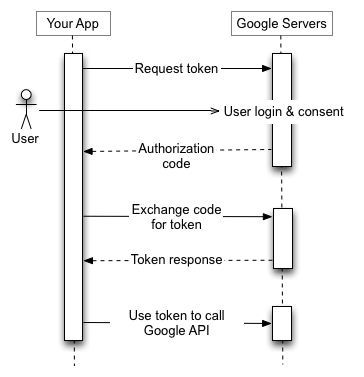
\includegraphics[width=0.7\textwidth]{oauthwebflow.png}
		\caption{OAuth web flow}\label{fig:oauth}
	\end{figure}

\section{Sequences}
Currently NARRA is still in development and many features and functions are not implemented yet, lates build doesn't provide a possibility to synchronize sequences between NARRA and our plug-in, so I would like to propose a way how it might be realized in future.

Sequence is structured way of describing which video clip should be taken and when it should be played on the timeline. One of the easiest and most popular ways to represent a sequence is to use \textbf{Edit decision list}.

\textbf{EDL} is a file format that is widely used by video editors, it consists from reel and timecode data that represents when and where each video clip should be used. Example of EDL file:
\begin{lstlisting}[caption=Part of EDL file, label=lst:lst_edl]
007  A004C018 V     C        00:00:20:16 00:00:22:14 00:02:00:07 00:02:02:05
* FROM CLIP NAME: A1B TK2
 
008  B004C011 V     C        16:47:08:10 16:47:11:08 00:02:02:05 00:02:05:03
* FROM CLIP NAME: B1B TK4
\end{lstlisting}
Adobe Premiere Pro provides a way to export and import EDL files, so we can use this possibility to synchronize sequences between our plug-in and NARRA. Basic scenario for sequence importing could be like this:
	\begin{enumerate}
		\item User double clicks on a sequence inside our application.
		\item Default browser launches and downloading of a chosen sequence starts.
		\item User imports downloaded EDL file using Adobe Premiere Pro built-in tools. 
	\end{enumerate}
In order to successfully import a sequence, all video clips that are used, have to be imported in advance, so that Adobe Premiere Pro can locate them.

Exporting of a sequence can be done similar way. For example, user could just upload EDL file directly from our plug-in into NARRA.

\section{Metadata}
Each project, library and item inside NARRA has an attached metadata to it. In our case, I can describe metadata as a set of \texttt{attribute} - \texttt{value}, where each attribute represents some piece of infromation about given element. For example, each project has name and description.

Set of metadata attributes is defined by vocabulary, one of the biggest vocabulary providers is \textbf{Dublin Core Metadata Initiative}.
\subsection{Dublin Core metadata standard}
The Dublin Core metadata standard is a simple yet effective element set for describing a wide range of networked resources.

The Dublin Core standard includes two levels: Simple and Qualified. Simple Dublin Core comprises fifteen elements; Qualified Dublin Core includes three additional elements (Audience, Provenance and RightsHolder), as well as a group of element refinements (also called qualifiers) that refine the semantics of the elements in ways that may be useful in resource discovery. 

The semantics of Dublin Core have been established by an international, cross-disciplinary group of professionals from librarianship, computer science, text encoding, the museum community, and other related fields of scholarship and practice.\cite{dublincore}

\subsection{NARRA metadata element set}
I would like to list metadata elements that are used by NARRA.

Every item's metadata contains a set of the following attributes:
	\begin{itemize}
		\item type
		\item name
		\item url
		\item library
		\item author
		\item thumbnail
		\item video\_proxy\_lq
		\item video\_proxy\_hq
		\item size
		\item duration
		\item timecode
		\item bitrate
		\item video\_codec
		\item colorspace
		\item resolution
		\item width
		\item height
		\item frame\_rate
		\item audio\_codec
		\item audio\_sample\_rate
		\item audio\_channels
		\item audio\_proxy
	\end{itemize}
To store metadata, Adobe Premiere Pro uses \textbf{Extensible Metadata Platform} standard. For each video footage, it creates \texttt{.xmp} file which specifies values for metadata elements. You can see a part of \texttt{.xmp} file in listing \ref{lst:xmp}.
\begin{lstlisting}[caption=Part of XMP file, label=lst:xmp]
<rdf:Description rdf:about=""
    xmlns:tiff="http://ns.adobe.com/tiff/1.0/">
   <tiff:Make>Canon</tiff:Make>
   <tiff:Model>Canon EOS 450D</tiff:Model>
   <tiff:Orientation>1</tiff:Orientation>
   <tiff:ImageWidth>4272</tiff:ImageWidth>
   <tiff:ImageLength>2848</tiff:ImageLength>
  </rdf:Description>
\end{lstlisting}

\subsection{Metadata synchronization with NARRA}
I would like to propose a model for metadata synchronization. Adobe Premiere Pro provides possibility to access \texttt{.xmp} files using ExtendScript. This way we can read those files, parse them and compare with data recieve from NARRA.

When user launches synchronization process, three situations may appear:
	\begin{enumerate}
		\item Element inside project bin doesn't have metadata specified (no XMP file). In this situation our plug-in should parse metadata received from NARRA, present this information as XML structured text and generate XMP file using ExtendScript functions.
		\item Element inside project bin has metadata assigned, but it differs from one that inside NARRA. In that case our plug-in should parse received data and change corresponding fileds inside XMP file.
		\item Element inside project bin has metadata assigned and values are the same as inside NARRA. In that case our plug-in shouldn't do anything.
	\end{enumerate}
\chapter{Paradigm shift}
At first glance we thought that Creative Suite version of Adobe Premiere Pro with provided SDK will be enough to implement desired functionality of the plug-in, but we encountered a problem with operating multiple files in project bin. There is no possibility to realize correct importing of project files into Adobe Premiere Pro CS5.5, so we decided to completely shift our paradigm and choose different approach to problem solving. We understand that we lose the flexibility of C language and possibility of usage many different frameworks and libraries, but in order to realize our needs it is necessary.

From this point we are switching from Adobe Premiere Pro CS5.5 version to CC 2014 version, that means:
	\begin{itemize}
		\item Adobe Premiere Pro SDK no longer needed, Panel SDK will be used.
		\item We are switching from development in C to development in JavaScript and ExtendScript, because CC 2014 version of Adobe Premiere Pro uses Chromium web browser for execution of plug-ins.
		\item All communication with Adobe Premiere Pro will be carried by ExtendScript functions.
		\item We no longer need to make two separate plug-ins for importing and exporting libraries and items from NARRA. We are going to make it as a single plug-in that will be synchronizing elements on local machine with elements in NARRA storage. 
	\end{itemize}
\section{Adobe Premiere Pro CC}
Creative Cloud (CC) version of Adobe products is the successor to Creative Suite that we chose as our working environment before encountering a problem. Adobe Premiere Pro CC allows us to use Panel SDK that provides much more functionality in comparison with SDK for Creative Suite version of video editing tool. 

Adobe announced that it will no longer release any products of CS version\cite{CC}, so choosing CC we also looking to the future. 

\subsection{Overview}
Adobe Premiere Pro is a timeline-based video editing software application. It is part of the Adobe Creative Cloud, which includes video editing, graphic design, and web development programs.

Premiere Pro has been used to edit feature films, such as Gone Girl, Captain Abu Raed, and Monsters, and other venues such as Madonna's Confessions Tour.\cite{adobe}
	\begin{figure}
		\centering
		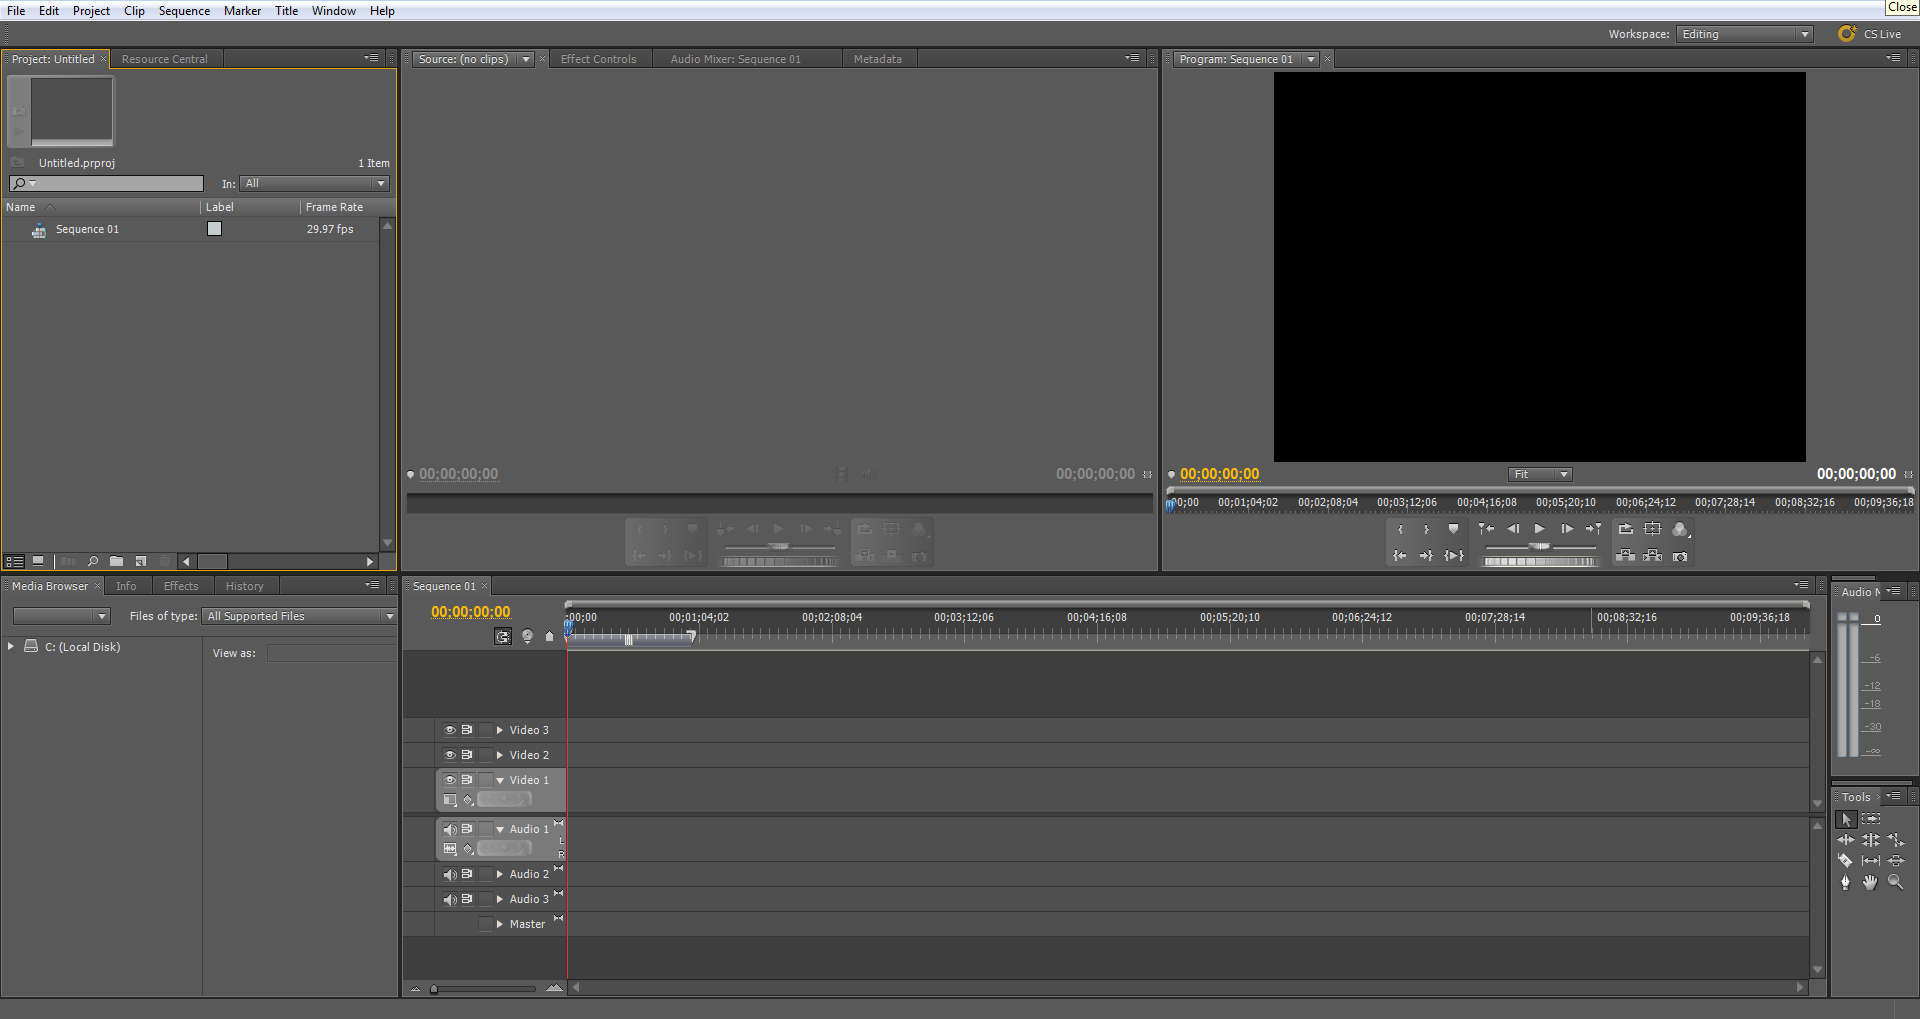
\includegraphics[width=1.1\textwidth]{PremiereMain.png}
		\caption{Adobe Premiere Pro CS5.5 window}\label{fig:APPWindow}
	\end{figure}
\subsection{History}
Premiere Pro is the redesigned successor to Adobe Premiere, and was launched in 2003. Premiere Pro refers to versions released in 2003 and later, whereas Premiere refers to the earlier releases. Premiere was one of the first computer-based NLEs (non-linear editing system), with its first release on Mac in 1991. Up until version Premiere Pro 2.0 (CS2), the software packaging featured a galloping horse, in a nod to Eadweard Muybridge's work, "Sallie Gardner at a Gallop".\cite{adobe}
	
Adobe Premiere Pro CC 2014 uses built-in web browser for executing plug-ins, so that means that we can use standard tools for web development to implement our plug-in.

\section{ExtendScript}
ExtendScript is a programming language, that is used for scripting Adobe products. We will use it as a layer between our plug-in and Adobe Premiere Pro since it can operate functions of this software directly. It has similar structure and syntax with JavaScript, but also very limited functionality. Extend script is a language that implemented according to Ecma standard, while JavaScript currently follows its own path and that creates troubles sometimes when we try to use them together. 
\subsection{ECMAScript}
This Ecma Standard is based on several originating technologies, the most well known being JavaScript (Netscape) and JScript (Microsoft). The language was invented by Brendan Eich at Netscape and first appeared in that company’s Navigator 2.0 browser. It has appeared in all subsequent browsers from Netscape and in all browsers from Microsoft starting with Internet Explorer 3.0.

ECMAScript is an object-oriented programming language for performing computations and manipulating computational objects within a host environment. ECMAScript is not intended to be computationally self-sufficient; indeed, there are no provisions in this specification for input of external data or output of computed results. Instead, it is expected that the computational environment of an ECMAScript program will provide not only the objects and other facilities described in this specification but also certain environment-specific host objects, whose description and behaviour are beyond the scope of this specification except to indicate that they may provide certain properties that can be accessed and certain functions that can be called from an ECMAScript program.

A \textbf{scripting language} is a programming language that is used to manipulate, customise, and automate the facilities of an existing system. In such systems, useful functionality is already available through a user interface, and the scripting language is a mechanism for exposing that functionality to program control. In this way, the existing system is said to provide a host environment of objects and facilities, which completes the capabilities of the scripting language. A scripting language is intended for use by both professional and non-professional programmers.

	\begin{itemize}
\item ECMAScript is object-based: basic language and host facilities are provided by objects, and an ECMAScript program is a cluster of communicating objects. An ECMAScript object is a collection of properties each with zero or more attributes that determine how each property can be used - for example, when the Writable attribute for a property is set to false, any attempt by executed ECMAScript code to change the value of the property fails. Properties are containers that hold other objects, primitive values, or functions. A primitive value is a member of one of the following built-in types: Undefined, Null, Boolean, Number, and String; an object is a member of the remaining built-in type Object; and a function is a callable object. A function that is associated with an object via a property is a method.
\item ECMAScript defines a collection of built-in objects that round out the definition of ECMAScript entities. These built-in objects include the global object, the Object object, the Function object, the Array object, the String object, the Boolean object, the Number object, the Math object, the Date object, the RegExp object, the JSON object, and the Error objects Error, EvalError, RangeError, ReferenceError, SyntaxError, TypeError and URIError.
\item ECMAScript also defines a set of built-in operators. ECMAScript operators include various unary operations, multiplicative operators, additive operators, bitwise shift operators, relational operators, equality operators, binary bitwise operators, binary logical operators, assignment operators, and the comma operator.
\item ECMAScript syntax intentionally resembles Java syntax. ECMAScript syntax is relaxed to enable it to serve as an easy-to-use scripting language. For example, a variable is not required to have its type declared nor are types associated with properties, and defined functions are not required to have their declarations appear textually before calls to them.\cite{ecma}
	\end{itemize}

\chapter{Design}
In this chapter I would like to describe process of designing user interface and structure of my application.
\section{User interface}
User interface is a layer that will "connect" user and application logic together. That's why I think that good user interface is almost a half of success of any application. 

While designing my user interface I was evaluating it by these criteria:
	\begin{description}
		\item [Clarity] Clarity is the most important element of user interface design. Indeed, the whole purpose of user interface design is to enable people to interact with your system by communicating meaning and function. If people can’t figure out how your application works or where to go they’ll get confused and frustrated. \cite{ui}
		\item [Familiarity] Familiar is something which appears like something else you’ve encountered before. When you’re familiar with something, you know how it behaves - you know what to expect.
		\item [Responsiveness] Responsive means a couple of things. First of all, responsive means fast. The interface, if not the software behind it, should work fast. Waiting for things to load and using laggy and slow interfaces is frustrating. Seeing things load quickly, or at the very least, an interface that loads quickly improves the user experience.

Responsive also means the interface provides some form of feedback. The interface should talk back to the user to inform them about what’s happening. \cite{ui}
	\end{description}
\subsection{Login page}
The main challenge for me while designing login page was how to place interactive elements more effectively, so that interface will have a good usability.

As I described earlier, user has two ways of authorization: 
	\begin{itemize}
		\item Using Google account
		\item Using Github account
	\end{itemize}
So I decided to make two buttons with icons of Google and Github respectively and provide a name of the service under it for those, who is unfamiliar with these icons.

Next element is the input field for a token, that user will copy from browser window. I placed it on a next row right after buttons, wanting to show that it is the next step in the login process. After all of it, there is a login button.

Overall look of the login page is shown on the figure \ref{fig:login}.
	\begin{figure}
		\centering
		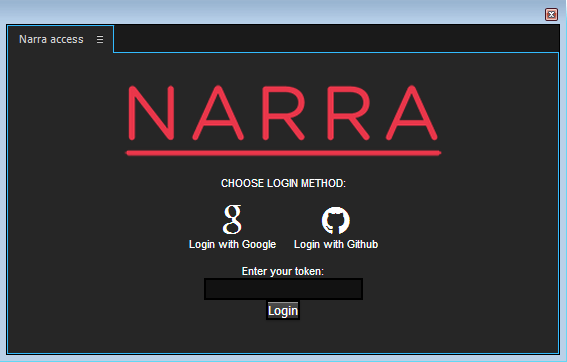
\includegraphics[width=0.9\textwidth]{LoginPage.png}
		\caption{Login screen of the plug-in}\label{fig:login}
	\end{figure}
\subsection{Project list}
For each project I decided to display it's name and thumbnails. At first, I wanted to display a grid, where each cell will represent a project, name will be inside a cell and background of a cell will be it's thumbnail. If you hover a cursor above the cell, it's background will change every second looping through thumbnail images.

In the end I decided to display a project as a strip, where you can see all thumbnail at once with a name below it. I think it is more convenient for user and more efficient for a workflow, user doesn't need to wait images to change to get what this project is about, all of them will be visible immediately.

On top of the screen you can see username of a logged in user, NARRA logo and a logout button. Below it there are buttons for navigating to project list and to list of libraries, also there is a search input form.

Final design of a project list you can see on figure \ref{fig:projects}
	\begin{figure}
		\centering
		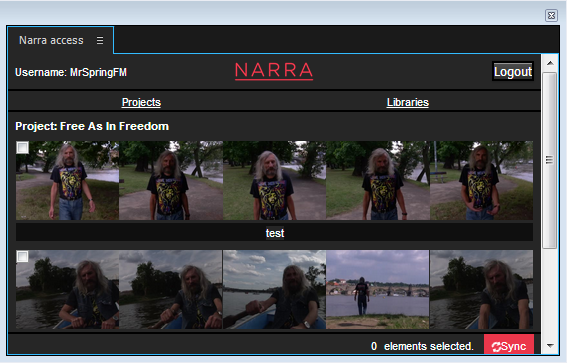
\includegraphics[width=0.9\textwidth]{libraries.png}
		\caption{List of libraries}\label{fig:libraries}
	\end{figure}
\subsection{List of items}
To visualize a list of items I decided to use tiles. After playing with layouts, I figured out that four tiles in a row is the optimal amount, because it is big enough and utilizes space efficiently at the same time. Below every tile I placed name of the item. I will use the same layout for displaying search results.
\chapter{Implementation}
\section{Application architecture}
Architecture of this plug-in is not complicated, best practices for web development were used, basically we are dealing with front-end development workflow. I this case, I decided to split different views into different HTML files:
	\begin{description}
		\item [index.html] This is the markup of the login screen that user sees after launching plug-in.
		\item [projects.html] File containing markup of project list.
		\item [libraries.html] File containing markup of list of libraries.
		\item [items.html] File containing markup of list of items.
	\end{description}
Application logic I decided to split into several JavaScript files:
	\begin{description}
		\item [ApiCalls.js] There are definitions of a functions that execute AJAX requests to NARRA.
		\item [Ui.js] File containing functions that manipulate with user interface, like content generation.
		\item [Premiere.jsx] File containing functions that communicate directly with Adobe Premiere Pro.
	\end{description}
In the next section I would like to describe implementation of somel key functionalities that specified in requirements.
\section{Realization of application logic}
\subsection{Authorization}
Lets describe the very first process that user will go through. On the figure \ref{fig:seq_auth} you can see a sequence diagram of a process where user goes through authorization and after it receives a token that will be used for communication with NARRA.
	\begin{figure}
		\centering
		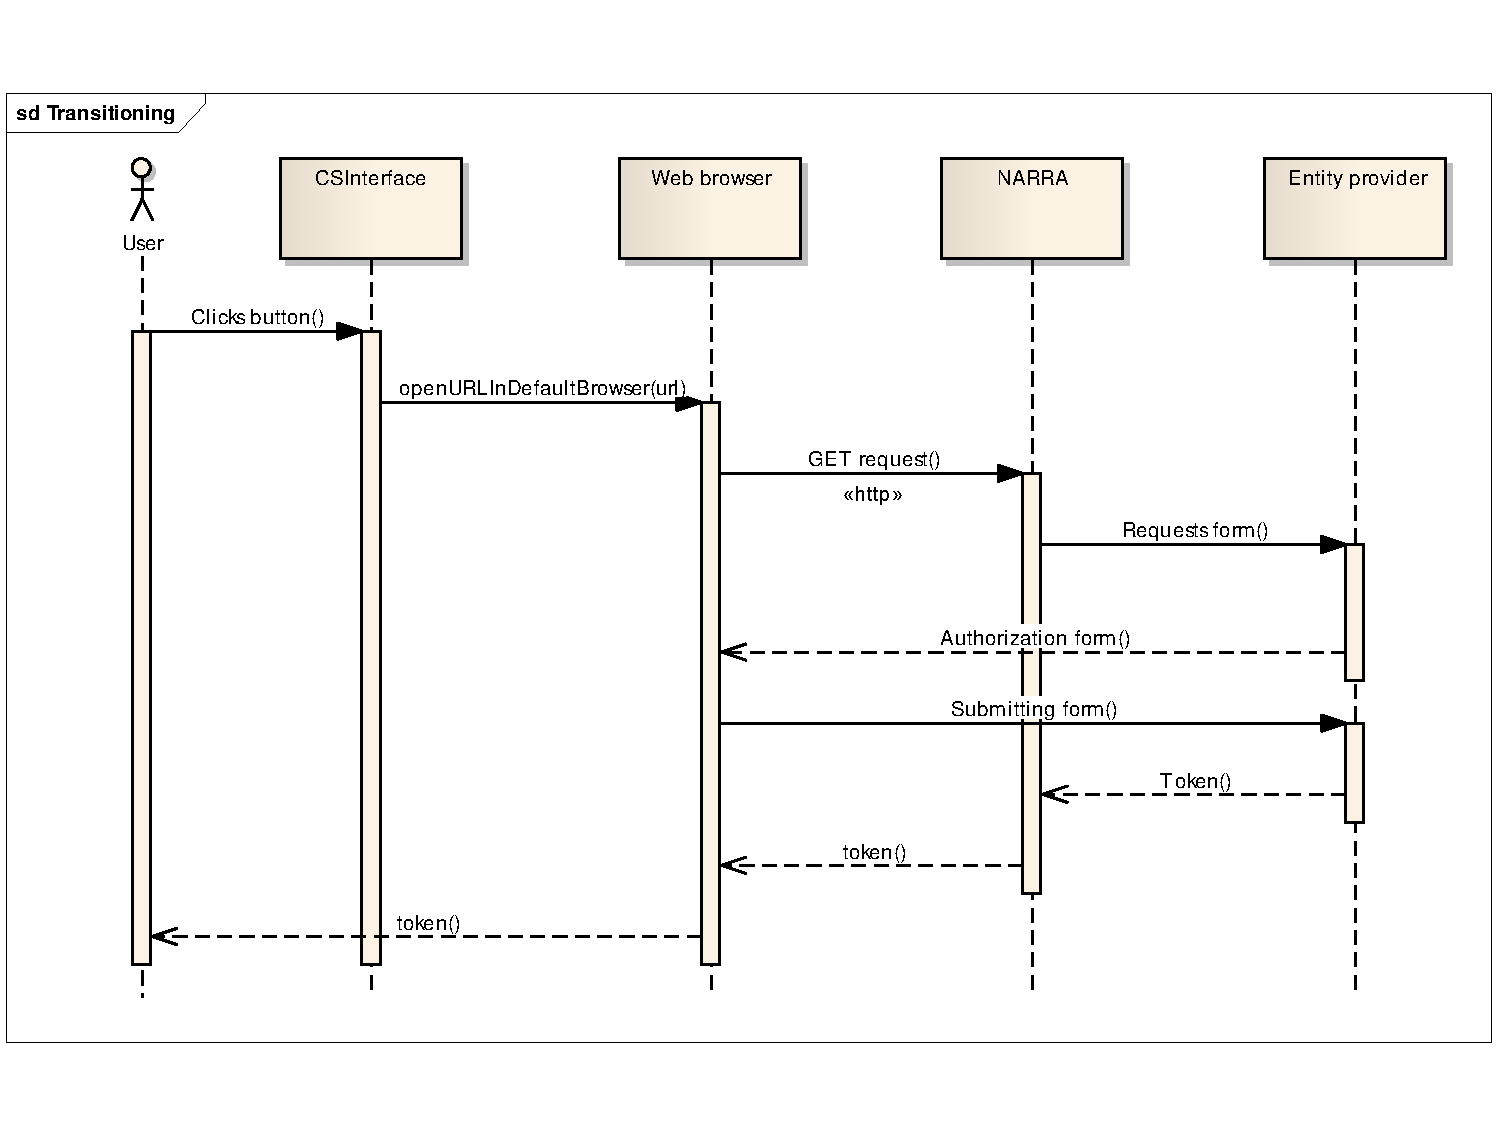
\includegraphics[width=1\textwidth]{AuthSeqDiag.pdf}
		\caption{Sequence diagram of authorization process}\label{fig:seq_auth}
	\end{figure}

Key function there is \texttt{openURLInDefaultBrowser(url)}. It is the method of \texttt{CSInterface} class, provided by Panel SDK. Execution of this method results in the opening of default browser and sending GET request to provided url.
\subsection{Displaying project list}
This process starts with a press of a button and resulting in displaying of the list of a projects inside our plug-in. You can see sequence diagram on the figure \ref{fig:seq_project}.
	\begin{figure}
		\centering
		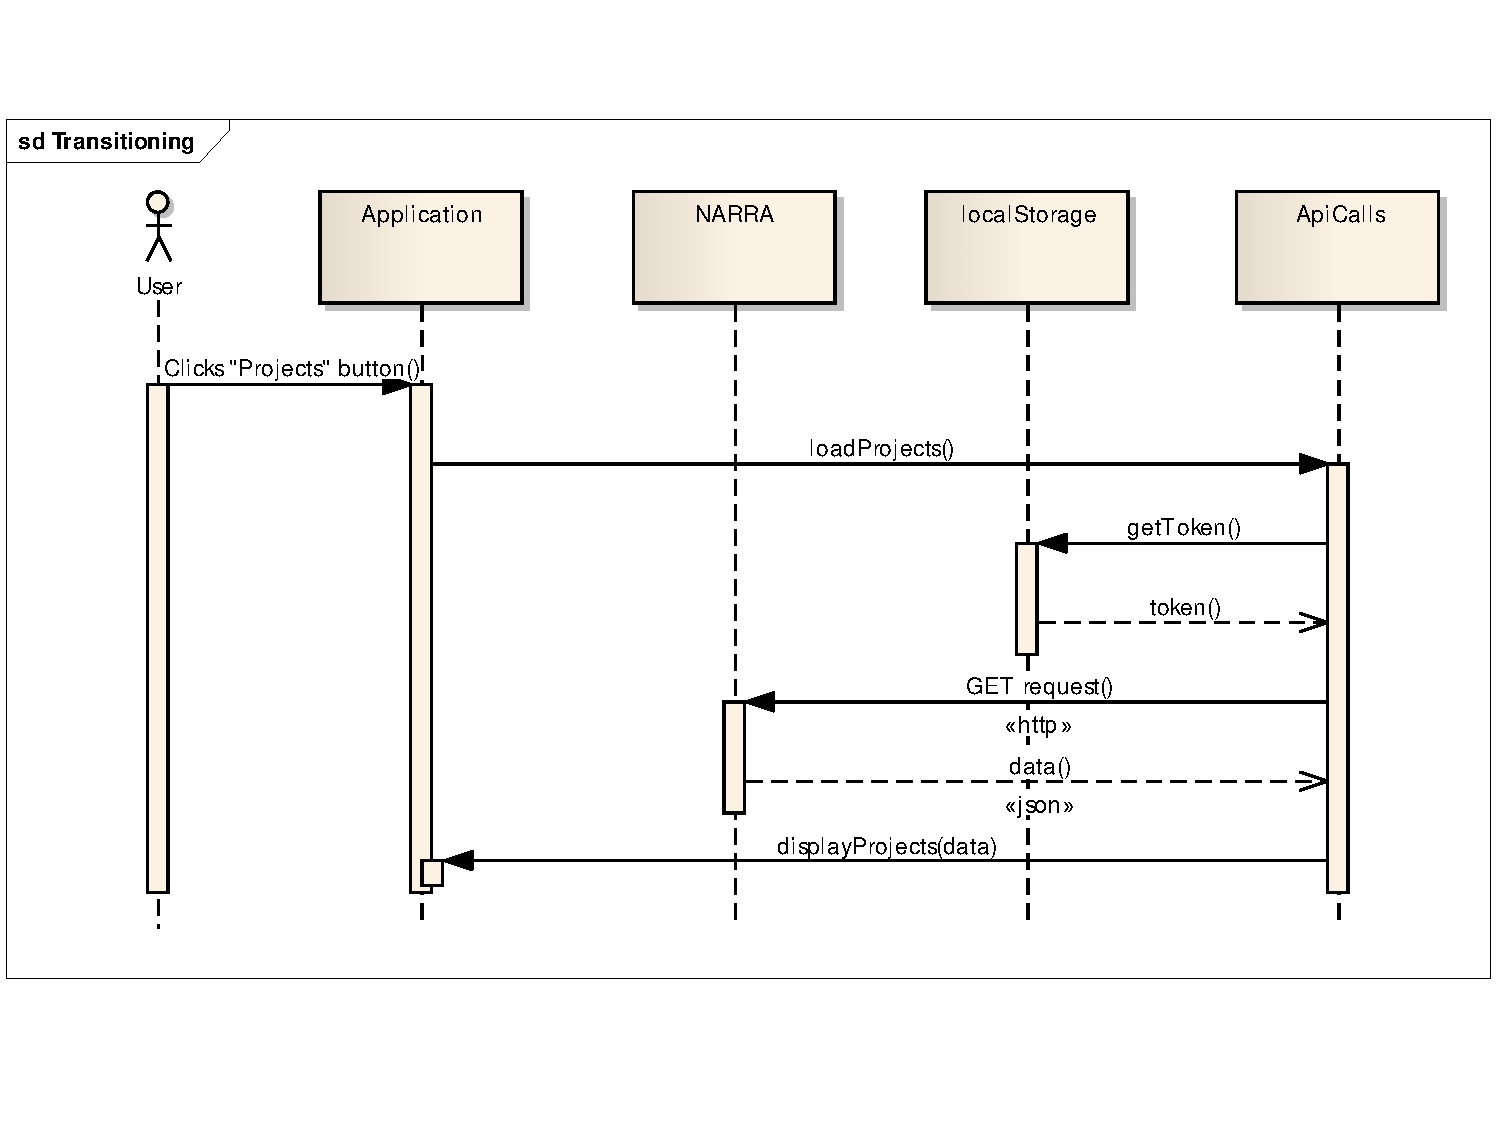
\includegraphics[width=1\textwidth]{ProjectsSeqDiag.pdf}
		\caption{Sequence diagram of getting projects list process}\label{fig:seq_project}
	\end{figure}

I decided to use \texttt{localStorage} as a storage for access token. LocalStorage is a new feature from HTML5 specification. It allows to store data (access token in my case) inside browser for later use.

The key functions in this process are \texttt{loadProjects()} and \texttt{displayProjects(data)}. 

Function \texttt{loadProjects()} is a "wrapper" around JQuery AJAX request, that is executed by \texttt{\$.ajax()} function. You can see implementation of it on listing \ref{lst:lst_loadProjects}.

Function \texttt{loadProjects(data)} is a function that takes JSON object, parses it and generates HTML content that will be inserted into \texttt{<div></div>} block and displayed to a user.
\begin{lstlisting}[caption=loadProjects() function, label=lst:lst_loadProjects]
function loadProjects() {
  $.ajax({
    method: "GET",
    url: url + "v1/projects?token=" + localStorage["token"],
    dataType: "json",

    success: function(msg) {
      displayProjects(msg);
    },
    error: function() {
      displayError("Cannot load projects.");
    }
  });
}
\end{lstlisting}

\subsection{Communication with Adobe Premiere Pro}
In order to communicate with Adobe Premiere Pro and to manipulate it's functions, we have to use ExtendScript programming language. Right now there is almost no information about this language available and it is poorly documented. I had to use samples provided by Adobe and figure out syntax and functions myself.

If we want to execute an ExtendScript function from our plugin, we have to use \texttt{evalScript(name, callback)} method, provided by CSInterface class and pass the name of the function with all it's parameters as a string. Callback function will get data returned after evaluating ExtendScipt function, there we can somehow work with it.

Example of code provided by Adobe:  
\begin{lstlisting}[caption=Evaluating createSequenceFromPreset function from sample panel, label=lst:lst_eval]
var csInterface = new CSInterface();
var path = csInterface.getSystemPath(SystemPath.EXTENSION);

if (path != null)
{
	path = path + '/payloads/PProPanel.sqpreset';
}
var pre = '$._ext_PPRO.createSequenceFromPreset(\'';
var post      = '\'';
var postpost  = ')';

var whole_megillah =  pre + path + post + postpost;
           	
csInterface.evalScript(whole_megillah);
\end{lstlisting}
As we can see, working with ExtendScript from JavaScript is not the most pleasant job. Also I want to mention process of passing arrays and objects from/to ExtendScript, it is very unconvenient and requires a lot of parsing, because all arrays and objects transform to strings.

I decided to implement synchronization mechanism using \texttt{sync()} function that crawls through project bins and collects ID's of items inside them. After it, array of ID's is returned back to our panel and processed by JavaScript, for each ID AJAX request is sent to NARRA to get information about each item inside project bin. After all information about items is received, array of item names is passed back to ExtendScript function \texttt{renameFootage()}, which renames items according to their names in NARRA.

\chapter{Testing}
Tests are very important in software engineering process, they demonstrate if application met the requirements and help in revealing problems and bugs.

Our application consists mostly from user interface with some application logic, I will describe testing process of these parts in next sections.
\section{User interface}
User interface is one of the most important parts of our plug-in, it should be very intuitive and clear, so that it won't confuse user or slow his/her workflow.

First of all, as was specified in requirements, application should integrate into Adobe Premiere Pro interface seamlessly, mimic it's style and has the same color schemes. I tried to manipulate appearance settings using built-in tools, our plug-in was changing colors and fonts accordingly.

Also responsiveness or our user interface was tested, plug-in was launched on different screen sizes, layout always remained the same. User gets visual notifications when time-consuming process is launched (rotating icon when synchronization of metadata is started). 
\section{Business logic}
For business logic testing I used real use cases:
	\begin{itemize}
		\item Authorization and logout.
		\item Browsing projects/libraries/items.
		\item Synchronization of items metadata.
	\end{itemize}
For the last one, we prepared \texttt{.zip} archive containing four footages from NARRA. We imported extracted files into Adobe Premiere Pro project bin and synchronized names of files with NARRA.

Our application passed all functional tests and fulfilled the requirements.
\setsecnumdepth{part}
\chapter{Conclusion}
Result of this thesis is working plug-in for Adobe Premiere Pro that fulfills the requirements. It allows users to browse projects, libraries and items inside NARRA and to synchronize metadata of items. While working on this thesis I've encountered various problems and complications, result of the biggest one is complete changing of working environment - we switched from developing in C++ using Adobe Premiere Pro SDK to Panel SDK and Web development workflow with JavaScript and ExtendScript as the main players. 

This plug-in can be used as a basis for future extensions, to fully utilize all possibilities of NARRA when something new will be added to the system. 

This project tought me how to quickly find solutions for arising problems, lack of ExtendScript documentation forced me to learn this language by analyzing source codes of different applications that are written in it. I have gained valuable experience and improved my technical skills.

\bibliographystyle{iso690}
\bibliography{Bibliography}

\setsecnumdepth{all}
\appendix

\chapter{User guide}


\chapter{Acronyms}
% \printglossaries
\begin{description}
	\item[GUI] Graphical user interface
	\item[SDK] Software Development Kit
	\item[API] Application programming interface
	\item[HTTP] Hypertext Transfer Protocol
	\item[URL] Uniform resource locator
	\item[CSS] Cascading Style Sheets
	\item[HTML] HyperText Markup Language
	\item[JSON] JavaScript Object Notation
	\item[EDL] Edit decision list
	\item[XML] Extensible Markup Language
	\item[PDF] Portable Document Format
	\item[JPEG] Joint Photographic Experts Group
	\item[REST] Representational state transfer
	\item[UI] User interface
	\item[XMP] Extensible Metadata Platform
\end{description}


\chapter{Contents of enclosed CD}

%change appropriately

\begin{figure}
	\dirtree{%
		.1 readme.txt\DTcomment{the file with CD contents description}.
		.1 exe\DTcomment{the directory with executables}.
		.1 src\DTcomment{the directory of source codes}.
		.2 wbdcm\DTcomment{implementation sources}.
		.2 thesis\DTcomment{the directory of \LaTeX{} source codes of the thesis}.
		.1 text\DTcomment{the thesis text directory}.
		.2 thesis.pdf\DTcomment{the thesis text in PDF format}.
		.2 thesis.ps\DTcomment{the thesis text in PS format}.
	}
\end{figure}

\end{document}
